\begin{figure}[H]
\centering
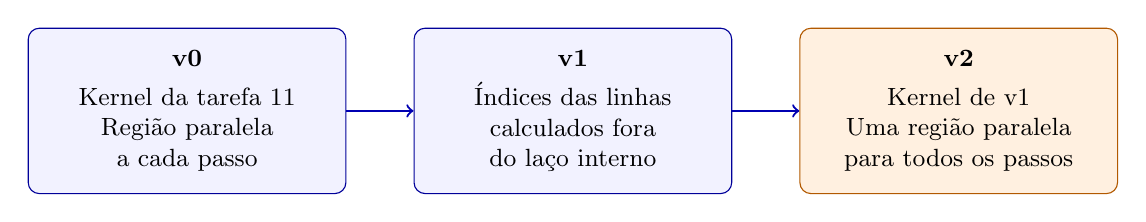
\begin{tikzpicture}[
  bloco/.style={draw=blue!60!black,fill=blue!5,rounded corners,
                text width=3.8cm,minimum height=2.1cm,align=center,font=\small},
  seta/.style={->,thick,blue!70!black}]
\node[bloco] (a) at (0,0) {\textbf{v0}\\[3pt]Kernel da tarefa 11\\Região paralela\\a cada passo};
\node[bloco] (b) at (4.9,0) {\textbf{v1}\\[3pt]Índices das linhas\\calculados fora\\do laço interno};
\node[bloco,fill=orange!12,draw=orange!70!black] (c) at (9.8,0)
{\textbf{v2}\\[3pt]Kernel de v1\\Uma região paralela\\para todos os passos};
\draw[seta] (a)--(b);
\draw[seta] (b)--(c);
\end{tikzpicture}
\caption{Evolução acumulada dos fontes. As três versões mantêm a mesma equação, a mesma ordem das operações por célula e o mesmo intervalo de medição.}
\label{fig:versoes}
\end{figure}
